%midterm1.tex
%%%%%%%%%%%%%%%%%%%%%%%%%%%%%%%%%%%%%%%%%%%%%%%%%%%%%%%%%%%%%%%%%%%%%%
%%%%%%            Math 403 Midterm \#1, Spring 2025             %%%%%%
%%%%%%                                                          %%%%%%
%%%%%%                 Instructor: Ezra Miller                  %%%%%%
%%%%%%%%%%%%%%%%%%%%%%%%%%%%%%%%%%%%%%%%%%%%%%%%%%%%%%%%%%%%%%%%%%%%%%
\documentclass[11pt]{article}

\oddsidemargin=17pt \evensidemargin=17pt
\headheight=9pt     \topmargin=26pt
\textheight=564pt   \textwidth=436.5pt
\parskip=1ex        %voffset=-6ex

\usepackage{amsmath,amssymb,graphicx,color,enumitem,tikz}
\setlist[enumerate]{parsep=1.5ex plus 4pt,topsep=0ex plus 4pt,itemsep=0ex}
  \setlist[itemize]{parsep=1.5ex plus 4pt,topsep=-1ex plus 4pt,itemsep=-1.33ex}

\leftmargini=5.5ex
\leftmarginii=3.5ex

%for \marginpar to fit optimally
%hoffset=-1.02in
\setlength\marginparwidth{2.2in}
\setlength\marginparsep{1mm}
\newcommand\red[1]{\marginpar{\linespread{.85}\sf%
		   \vspace{-1.4ex}\footnotesize{\color{red}#1}}}
\newcommand\score[1]{\marginpar{\vspace{-2ex}\color{blue}{#1/14}}\hspace{-1ex}}
\newcommand\extra[1]{\marginpar{\color{blue}{#1/1}}\hspace{-1ex}}
\newcommand\total[2]{\marginpar{\colorbox{yellow}{\huge #1/#2}}}
\newcommand\collab[1]{\marginpar{\vspace{-11ex}\colorbox{yellow}{#1/3}}\hspace{-1ex}}
\newcommand\magenta[1]{\colorbox{magenta}{\!\!#1\!\!}}
\newcommand\yellow[1]{\colorbox{yellow}{\!\!#1\!\!}}
\newcommand\green[1]{\colorbox{green}{\!\!#1\!\!}}
\newcommand\cyan[1]{\colorbox{cyan}{\!\!#1\!\!}}
\newcommand\rmagenta[2][0ex]{\red{\vspace{#1}\magenta{\phantom{:}}\,: #2}}
\newcommand\ryellow[2][0ex]{\red{\vspace{#1}\yellow{\phantom{:}}\,: #2}}
\newcommand\rgreen[2][0ex]{\red{\vspace{#1}\green{\phantom{:}}\,: #2}}
\newcommand\rcyan[2][0ex]{\red{\vspace{#1}\cyan{\phantom{:}}\,: #2}}

\newcommand\points{\makebox[0pt][r]{[14pts]\ }}

%For separated lists with consecutive numbering
\newcounter{separated}

\newcommand{\excise}[1]{}
\newcommand{\comment}[1]{{$\star$\sf\textbf{#1}$\star$}}

%%%%%%%%%%%%%%%%%%%%%%%%%%%%%%%%%%%%%%%%%%%%%%%%%%%
%                                                 %
% TO ENABLE GRADING, DO NOT ALTER ABOVE THIS LINE %
%                                                 %
%%%%%%%%%%%%%%%%%%%%%%%%%%%%%%%%%%%%%%%%%%%%%%%%%%%

%new math symbols taking no arguments
\newcommand\0{\mathbf{0}}
\newcommand\bb{\mathbf{b}}
\newcommand\ee{\mathbf{e}}
\newcommand\pp{\mathbf{p}}
\newcommand\vv{\mathbf{v}}
\newcommand\xx{\mathbf{x}}
\newcommand\yy{\mathbf{y}}
\newcommand\CC{\mathbb{C}}
\newcommand\FF{\mathbb{F}}
\newcommand\RR{\mathbb{R}}
\newcommand\Cb{\mathbf{C}}
\newcommand\Nb{\mathbf{N}}
\newcommand\Ec{\mathcal{E}}
\newcommand\Mc{\mathcal{M}}
\newcommand\Pc{\mathcal{P}}
\newcommand\Vc{\mathcal{V}}
\newcommand\GL{\mathrm{GL}}
\newcommand\from{\leftarrow}
\newcommand\ffrom{\longleftarrow}
\newcommand\goesto{\rightsquigarrow}

%redefined math symbols taking no arguments
\newcommand\<{\langle}
\renewcommand\>{\rangle}
\renewcommand\aa{\mathbf{a}}
\renewcommand\implies{\Rightarrow}

%to explain about LaTeX commands:
\newcommand\command[1]{\texttt{$\backslash$#1}}

%for easy 2 x 2 matrices
\newcommand\twobytwo[1]{\left[\begin{array}{@{}cc@{}}#1\end{array}\right]}

%for easy column vectors
\newcommand\colvec[1]{\left[\begin{array}{@{}c@{}}#1\end{array}\right]}

%replaces \atop
\newcommand{\aoverb}[2]{{\genfrac{}{}{0pt}{1}{#1}{#2}}}

%for overlines
\def\ol#1{{\overline {#1}}}


%%%%%%%%%%%%%%%%%%%%%%%%%%%%%%%%%%%%%%%%%%%%%%%%%%%%%%%%%%%%%%%%%%%%%%
\begin{document}%%%%%%%%%%%%%%%%%%%%%%%%%%%%%%%%%%%%%%%%%%%%%%%%%%%%%%
%%%%%%%%%%%%%%%%%%%%%%%%%%%%%%%%%%%%%%%%%%%%%%%%%%%%%%%%%%%%%%%%%%%%%%


\title{\mbox{}\\[-11.4ex]Math 403 Midterm \#1, Spring 2025\\\normalsize
	Instructor: Ezra Miller\\[-2.5ex]}
\author{[1pt] Solutions by: Thomas Kidane\\[1ex]
I verify that I have consulted no electronic or human sources except
those allowed\\
and that I have in all other ways complied with Duke's code of
academic honesty.\hfill\mbox{}\\[.5ex]
\ \ \ [1pt] Signature:- I agree}
\date{\mbox{}\\[-2.6ex]Due Date: 11:59pm Saturday 15 February 2025}

\maketitle
\thispagestyle{empty}%

\vspace{-5ex}%
\noindent
\textsc{Reading assignments}\total{}{100}%
\begin{enumerate}[itemsep=-1ex]\setcounter{enumi}{10}
\item%11.
for Thu.~13 February
  \begin{itemize}
  \item{}%
  [Treil, \S 6.1--\S 6.2] Spectral theorem, normal operators
  \end{itemize}

\item%12.
for Tue.~18 February
  \begin{itemize}
  \item{}%
  [Treil, \S 6.3.1--6.3.2] singular values, positive (semi)definite operators
  \item{}%
  [Lax, Appendix 10, Theorem 1, p.334--337] Schur factorization
  \item{}%
  [Lax, Chap.8: \S Spectral Resolution, \S Normal Maps]
  \item{}%
  [Lax, Chap.9: \S Polar Decomposition--\S Singular Value
  Decomposition, p.169--170]
  \end{itemize}
\end{enumerate}

\noindent
\textsc{Problems}

\begin{enumerate}
\item\ \score{}%1.
Let $C$ be a convex cone (Homework~\#2.11).  Prove that $0$ is an
extreme point of~$C$ if the cone~$C$ doesn't contain a straight line.
Construct a convex cone that contains an entire straight line but has
$0$ as an extreme point.

\textbf{Solution}

Let's prove the contrapositive, assume that 0 is an extreme point, therefore it is in the middle of the a line segment,
between $x$ and $y$, but since it is a cone, it must be closed under non-negative scaling, therefore
you can extend the line segment to infinty on both sides to get a line, which means there is a line if 0 is 
an extreme point, proving the statement.

The below construction is a counter example to the second part of the question.

\begin{center}
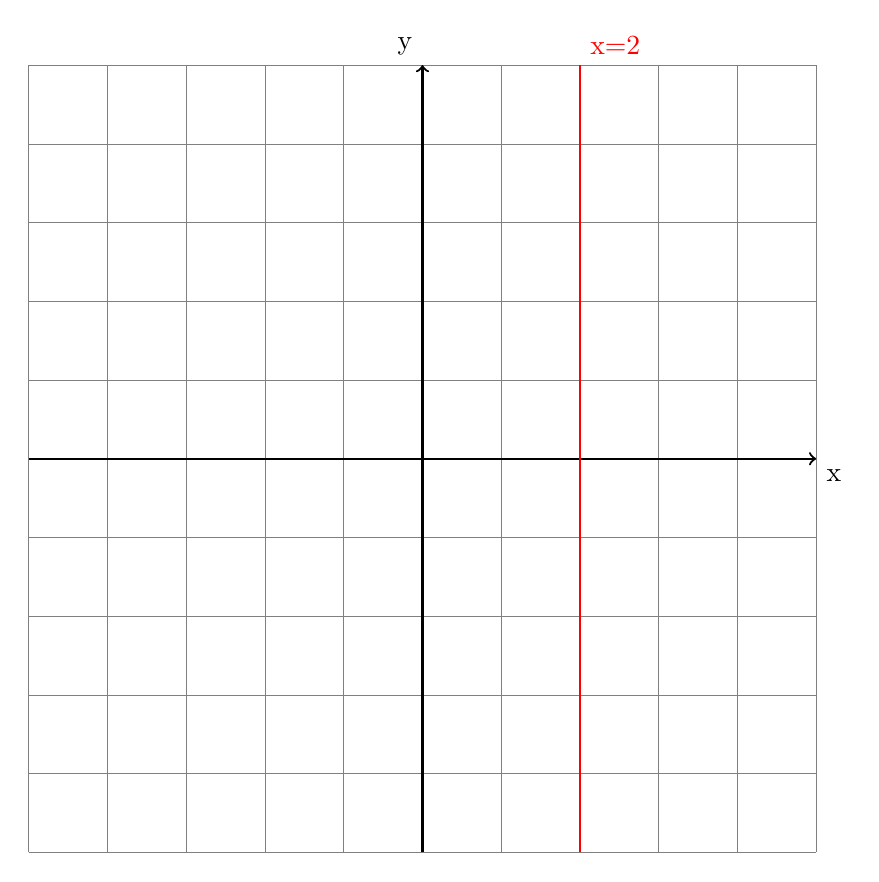
\begin{tikzpicture}
  % Draw the grid
  \draw[step=1cm,gray,very thin] (-5,-5) grid (5,5);

  % Draw the axes
  \draw[thick,->] (-5,0) -- (5,0) node[anchor=north west] {x};
  \draw[thick,->] (0,-5) -- (0,5) node[anchor=south east] {y};

  % Draw the vertical line at x=2
  \draw[red,thick] (2,-5) -- (2,5) node[anchor=south west] {x=2};
\end{tikzpicture}
\end{center}

All the points on the line $x=2$ are in the cone and all the non-negative scaling, but 0 isn't an extreme point, because
all the points are to the right of the y-axis and therefore the only way to have a line through,
0 is to have a line that is vertical, which is a impossible in this case.


\item\ \score{}%2.
Fix a finite field $\FF_q$ with $q$ elements.  Show that $q$ is a
power of a prime integer~$p$.  Hint: $\FF_q$ is a vector space over
$\FF_p$ for some prime~$p$; why is that true, and how is it useful?

\textbf{Solution}

For notational ease let's denote 2 as 1+1, 3 as 1+1+1, and so on. 
Where 1 is the multiplicative identity in the field. We know
that for finite fields the characteristic is a prime number(from homework 1). Another thing worth of note 
is that the inverses of all the elements listed are also inside this set.

\textit{Proof:} From number theory we can take take Bezout's identity to show that for
coprime integers $m,n$ there exists integers $a,b$ such that $am+bn=1$. In our situation
since the field operations can be constructed to resemble integer multiplicaiton and addition under modulo
we can see that $\exists n\in \{1,2,3,...,q-1\}, \exists m \in \mathbb{Z},  \;  \forall q \in \{1,2,3,...,p-1\}$
such that 

$$nq + mp = 1 \Rightarrow nq \equiv 1 \mod p \Rightarrow n^{-1} = q \wedge q \in \{1,2,3,...,p-1\}$$

Or simply stated each number has modulo inverse for a prime number $p$. So this set is closed both 
under addition and multiplication, and therefore constitutes a subfield.


If all the elements in  the broader field can be described as a linear combination of 1 we are done since $q=p$, 
else $\exists g$ such that $g$ is not a linear combination of 1.

We also can't describe $g+1$ as a linear combination of 1, since that would imply $g$ is a linear combination of 1
because $1,2,..., q-1$ are closed under addition and if $g+1$ were in this set then $g+1+q-1=g+0=g$ would 
also be in this set, which is a contradiction. Continuing this argument we can see that $g+1, g+2, ..., g+q-1$, 
are all distinct elements of the field. Along the same line of reasoning we can see that $g*1, g*2, ..., g*(q-1)$
are also not in any of the sets we have seen before because they are all closed under multiplication, therefore each
multiple of $g$ can be extended to make $p$ elemnents and therefore there are in total $p^2$ elements(corresponding to all the linear combinations of 1 and g) that we
have seen so far. We are also left with describing $g^2$, but there are really only few cases to consider, one is when $g^2$ is 1,
which is the case in which $g$ it its own inverse, if so then then the set we have described so far
is closed under multiplication and the hypothesis is correct.

Second is the case when it is not its own inverse, this case is broken up into two cases, one 
where $g^2$ can be described as a linear combination of $g$ and 1, in which case the set is still closed, 
under multiplication, otherwise $g^2$ is a completely different element than the ones we have seen before.

If $g^2$ is completely different than the elements we have seen before, then by extension all linear combination 
of $1, g, g^2$ are also different elements, pushing our size to $p^3$, we can progressivly increase 
the number of elements through this procedure until we reach a point when $g^y=1$. It is inevitable 
that in a finite field this must happen, because the set of elements is finite and we can't keep generating 
new elements forever, therefore we must reach a point when $g^y=1$.

At this point we have either exhausted all the elements in the field, or there is another element $x$ that 
can't be described as a linear combination of all the elments we have seen so far, but this 
is analogous to the argument above with the new element being $x$, and we can keep repeating this argument, each time increasing the number
of elements by a power of $p$, until we reach $q=p^n$.

Note: The main idea of my proof is that each time I encounter a new element that can't be described
as a linear combination of the elements I have seen so far, then it must increase the number of elmeents 
I have so far, by $p$. I tried to prove that the set $g, g+1, g+2,... , g+p-1$ is closed under multiplication,
but I couldn't prove it unless $g^{-1} = g$, I don't know if this claim is true or not, but I think it is 
true because when you have a chain of $g*g*g*...*g=1$, you can brake it up in the middle to get $g*g*...*g=(g*g*...*g)^{-1}$,
but this proof would rely on the chain of multiplication having even length, and I don't know if that is true or not for every finite field.

\pagebreak

\item\ \score{}%3.
Fix a $5 \times 5$ matrix~$A$ whose sole eigenvalue is~$\lambda$.
Either find the Jordan form of~$A$ assuming that $A - \lambda I$, $(A
- \lambda I)^2$, and $(A - \lambda I)^3$ have kernels of dimension
$2$, $3$, and~$5$, respectively, or else prove that no such matrix~$A$
exists.  \mbox{Justify your response either way}.

\textbf{Solution}

Theorem used:- $ker(A-\lambda I)^k -  ker(A-\lambda I)^{k-1}$ is the number of jordan blocks of at least size k.

\textit{Pf:} Prof. Miller said it in class, but I will just prove it here for myself and I can
get free feedback on my proof. The dimension of the kernel increases because generalized eigen vectors in each jordan
blocks are annihilated in each itereation, and in the each itereation the number of new generalized eigen vectors
that get annihilated corresponds to the number of jordan blocks that haven't annihilated all their 
generalized eigen vectors yet, so for an eigen vector to be annihilated in the $k^{th}$ iteration, it must be in the kernel of $(A-\lambda I)^k$ but not in the kernel of $(A-\lambda I)^{k-1}$. 
Therefore the size of the jordan block it corresponds to, must be atleast be size $k$.

Since the kernel of $A-\lambda I$ is 2, then there are 2 jordan blocks(All jordan blocks have size atleast 1). Since the kernel of
$(A-\lambda I)^2$ is 3, then only 1 jordan block has size $> 1$ because if both had 
size $> 1$, then the dimension kernel would increase by 2. So now we have that there are 
2 jordan blocks, one of size 1 and one of size at least 2. Since the sum the sizes of all 
jordan blocks must sum upto 5, then the size of the second jordan block must be 4. 

We hit the contradiction because the kernel of $(A-\lambda I)^3$ is 5. The increase in the dimension of the kernel is 2
but we already know that there is only one jordan block that is contributing additional dimensions to 
the kernel, and it can't contribute more than 1 dimension to the kernel, therefore no such matrix exists
(A matrix can't have 2 jordan blocks of size atleast 3 and 1 of size atleast 2).

\pagebreak
\item\ \score{}%4.
Suppose $\varphi: V \to W$ is an invertible linear transformation of
Hermitian inner product spaces.  Prove or construct a counterexample:
if $\ee_1,\ldots,\ee_n$ is an orthogonal basis of~$V$ and
$||\varphi(\ee_i)|| = ||\ee_i||$ for all~$i$, then $\varphi$ is
an~isometry: $||\varphi(\vv) - \varphi(\vv')|| = ||\vv - \vv'||$.

\textbf{Solution}

Counter Example

The matrix $\begin{bmatrix} 1/2 & \sqrt3/2 \\ \sqrt3/2 & 1/2 \end{bmatrix}$ satisfies  the condition above because
the image of the basis vectors has unit length but the norm isn't conserved $\sqrt{(\sqrt3/2 - 1/2)^2 + (\sqrt3/2 - 1/2)^2} \neq 1$.
\pagebreak

\item\ \score{}%5.
Fix vector spaces $W \subseteq V$ over a field~$F$.  Let $T: V \to V$
be a linear transformation such that $T(W) \subseteq W$.  Using the
universal property of quotients, prove that $T$ induces a linear
transformation $\ol T: V/W \to V/W$ given by $\ol T(v + W) = T(v) + W$.
Show further that $\ol T$ is an isomorphism if $T$ is an isomorphism
and $V$ has finite dimension.  Must the same hold if $V$ does not have
finite dimension?  Prove or give a counterexample.


\textbf{Solution}

All elements in $V$ can be expressed as $w + v$ where $w \in W$ and $v \in V/W$. Therefore
$\overline{\overline T} : V \rightarrow V/W$ defined by
$\overline{\overline T}(W+v) = T(v) + W$ is well defined, and its kernel is $W$, therefore by 
the universal property of quotients there exists a linear transformation ${\overline T}: V/W \rightarrow V/W$ such that
$\overline{T} (v + W) = T(v) + W$.

If $T$ is an isomorphism, then $\overline T(v_1+W) = \overline T(v_2+W) \rightarrow $ 
$T(v_1) + W = T(v_2) + W\\ \rightarrow T(v_1) = T(v_2)$, the value of $w$ doesn't matter,
 therefore the two elements in the codimension($V/W$) are the same, therefore $\overline T$ is injective
 and since the dimension of both domain and output spaces are the same, it is also surjective, therefore it is an isomorphism.


This proof doesn't work for Infinite dimensional case, because you need not have $T(W)=W$(The assumption
that w doesn't matter isn't valid in the infinite case, because it is not guaranteed that the preimage of w
is in W). For example assume you have a the set of basis $e_i \; \vert i\geq 0, \;  i\in \mathbb{Z}$. 
Define $W$ as the subspace spanned by the basis vector $e_i, i \equiv 0 \; mod \; 2$. Then 
$V/W$ is spanned by the odd standard vectors.

Define $T(v)$ that maps $e_i$ to $e_{i+2}$ if \textit{i} is even; $e_1$ to $e_0$; and everything else 
to $e_{i-2}$. $T$ satifies all the properties($T(W) \subseteq W$) and is an isomorphism but $\overline T$ is not an isomorphism, because $e_1$ is mapped to 0, therefore 
$\overline T$ has a non-empty kernel, therefore the statement doesn't hold in an infinite dimensional case.
\pagebreak

\item\ \score{}%6.
Fix integers $0 < d < e < n$.  Express $\{\text{chains } V_d \subseteq
V_e\}$ of subspaces of~$F^n$ of dimensions $d$ and~$e$ as a quotient
of~$\GL_n(F)$ modulo a subgroup.  How many such chains are there if $F
= \FF_q$ is a field with $q$ elements?




\textbf{Solution}

The set of chains can be expressed as the quotient of $\GL_n(F)$ 
module the subgroup that fix $V_d$ and $V_e$. This subgroup is $R_d^e$. Where
$R_d^e$ is the set of matrices where, there is an invertible $d \times d$ matrix in the 
top left corner of the $n \times n$ matrix, an invertible $(e-d) \times (e-d)$ matrix in the middle("starting from the d+1 row and column and ending at the e row and column"), followed by an $ (n-e) \times (n-e)$
invertible matrix in the bottom right corner, and everything else is 0. 

\begin{align*}
    R_d^e &= \begin{bmatrix} A & 0 & 0 \\ 0 & B & 0 \\ 0 & 0 & C \end{bmatrix} \; \: \text{Where A is $d \times d$, B is $(e-d)\times (e-d)$, C is $ (n-e)\times (n-e)$}\\
    \GL_n(F)/R_d^e &= \{\text{Chains } V_d \subseteq V_e\}
\end{align*}

Why is this true? Because multiplicaiton by $R_d^e$ from the right maintains the subspace of the 
left $d$ columns and the left $e$ columns, as well, therefore $V_d$ and $V_e$ stay constant, where 
$V_d$ is the span of the first $d$ columns and $V_e$ is the span of the first $e$ columns. So you can make 
a bijection between the set of chains and the set of cosets of $R_d^e$ in $\GL_n(F)$, because each coset 
only describes one chain and each chain can be described by a coset.

From the last homework we know that the number of invertible matrices 
of size $n$ in a finite field of size $q$ are $\prod_{i=0}^{n-1} (q^n - q^i)$. So we get
$\frac{\prod_{i=0}^{n-1} (q^n - q^i)}{\prod_{i=0}^{d-1} (q^d - q^i) \cdot \prod_{i=0}^{e-d-1} (q^{e-d} - q^i) \cdot \prod_{i=0}^{n-e-1} (q^{n-e} - q^i)}$.
\pagebreak

\item\ \score{}%7.
Is the $\infty$-norm $\Vert \cdot \Vert_\infty$ on~$\RR^n$ induced by
an inner product?  Justify your response.

\textbf{Solution}

No, there is no such inner product that induces the infinity norm.

\textit{Proof:} Assume that there is some norm $v$ that induces the infinity norm on $n=2$.

\begin{align*}
    v(x,x) &= \max(|x_1|, |x_2|)\\
\end{align*}
Let's find a contradiciton with the norm of $(3,2)$.
\begin{align*}
    v((3,2),(3,2)) &= \max(|3|, |2|) = 3\\
    v((3,2),(3,2)) &= v((2,0),(3,2)) + v((1,2),(3,2)) \; \: \text{By Linearity} \\
    &= 2*v((2,0),(2,0)) + 2*v((1,2),(1,2)) = 4 + 4 \neq 3  \; \: 
\end{align*}

Since we didn't assume anything about $v$ then the contradiction exists for any function that 
is an inner product, therefore there is no inner product that induces the infinity norm.
\end{enumerate}
\end{document}

%%% Various Emacs customizations:
%%% Local Variables:
%%% fill-column: 70
%%% indent-tabs-mode: t
%%% TeX-electric-sub-and-superscript: nil
%%% TeX-brace-indent-level: 0
%%% LaTeX-indent-level: 0
%%% LaTeX-item-indent: 0
%%% End:
